%!TEX root = ../Thesis.tex
%Chapter 1

\chapter{Asymmetric scattering by non-Hermitian potentials}
\label{Chapter1}
\lhead{Chapter 1. \emph{Asymmetric scattering by non-Hermitian potentials}}
%
\null
% \vfill
\textit{``You must unlearn what you have learned.''}
\begin{flushright}
  {\bf Master Yoda}\\
  The Empire Strikes Back
\end{flushright}
% \vfill
\null

In this chapter I study the properties of potentials with asymmetric transmission or reflection for a quantum, spinless particle of mass $m$ satisfying a one-dimensional (1D) Schr\"{o}dinger equation. I propose six types of asymmetric devices according to the asymmetries of the transmission/reflection coefficients, see fig. \ref{fig:chapter1_cases}. Non-Hermitian and non-local potentials will be necessary to construct this kind of devices, therefore an important part of this chapter will consist in studying their properties. In particular their behaviour with respect to symmetries such as parity, time-reversal and PT. Symmetries can be used, analogously to their standard application in atomic physics to determine selection rules for allowed/forbidden transitions, to predict whether a certain potential may or may not lead to asymmetric scattering. The concept of symmetry, however, must be generalized when dealing with non-Hermitian potentials.

The theory in this chapter is worked out for particles and the Schr\"odinger equation but it is clearly of relevance for optical devices
due to the much exploited analogies and connections between Maxwell's equations and the Schr\"odinger equation,
which were used, e.g., to propose  the realization of PT-symmetric potentials in optics \cite{Ruschhaupt2005}.

The rest of the chapter goes as follows. In sections \ref{sec:chapter1_ScattFormalism} and \ref{sec:chapter1_LeftAndRightEigenstates} I introduce the basics of scattering formalism and the concept of left/right eigenvectors, which will be fundamental to understand the rest of the chapter. In section \ref{sec:chapter1_generalizedSymmetries} the concept of symmetry will be generalized for non-Hermitian Hamiltonians. A set of selection rules will be derived for the scattering coefficients. In section \ref{sec:chapter1_AsymmetricDevices} I will describe the 6 types of asymmetric devices and how the different selection rules from the generalized symmetries of the Klein 4-group (composed by the identity, parity, time reversal and PT-symmetry) affect them. In section \ref{sec:chapter1_examples} some examples of non-local potentials leading to asymmetric scattering are given. In section \ref{sec:chapter1_extension} I give an example of a local PT potential that has completely asymmetric reflection in a broad range of incident momenta. Finally, in section \ref{sec:chapter1_Discussion} I summarize the main results of this chapter.

\begin{figure}
  \center
  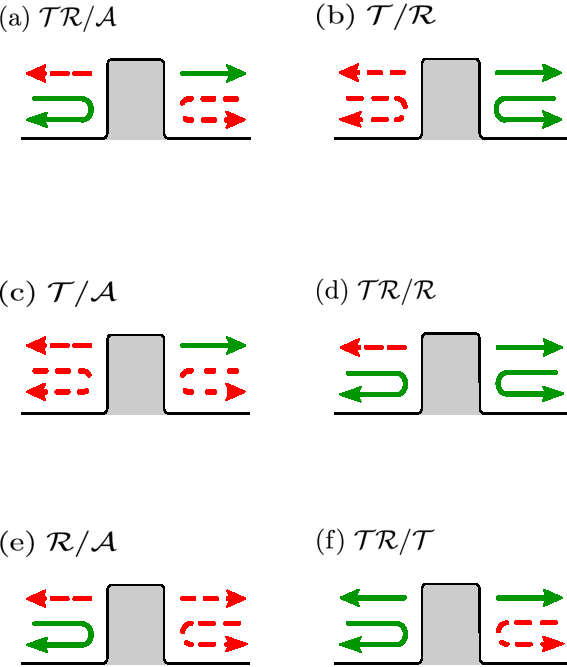
\includegraphics[width = 0.5\linewidth]{Figures/PotentialCasesPT.pdf}
  \caption{Devices with asymmetric scattering (limited to scattering coefficients being 0 or 1).  The dashed and continuous lines represent respectively zero or one
  for the moduli of the scattering amplitudes; the bended lines are for reflection amplitudes, and the straight lines for transmission:
  (a) One-way mirror ($\cal{TR/A}$); (b) One-way barrier ($\cal{T/R}$); (c) One-Way T-filter ($\cal{T/A}$);
  (d) Mirror \& 1-way transmitter ($\cal{TR/R}$); (e) One-way R-filter ($\cal{R/A}$); (f) Transparent, one-way
  reflector ($\cal{TR/T}$). The nomenclature for the devices is explained in the main text of section \ref{sec:chapter1_AsymmetricDevices}
  % The letter codes summarize the effect of left and right incidence, separated by a  slash ``$/$''.
  % ${\cal T}$ or ${\cal R}$ on one side of the slash indicate a unit
  % transmission or reflection coefficient
  % for  incidence from that side, whereas the absence of one or the other letter corresponds to zero coefficients.
  % An ${\cal A}$ denotes ``full absorption'', i.e., both moduli of reflection and transmission amplitudes are zero for incidence from one side.
  % For example,  $\cal{TR/A}$ means unit modulus transmission
  % and reflection from the left and total absorption from the right.
  \label{fig:chapter1_cases}}
\end{figure}

\section{Non-Hermitian scattering in 1 dimension \label{sec:chapter1_ScattFormalism}}

In this section I will put together a minimum set of ideas and tools needed to describe scattering in 1 dimension. The ideas in this section can be found with more detail in \cite{Muga2004}, which generalizes the results in the celebrated book by Taylor \cite{Taylor1972} to non-Hermitian Hamiltonians. In scattering theory one deals with the Hamiltonian for a particle of mass $m$ subjected to the action of a potential $V$
%
\begin{equation}
  H =  H_0 + V,
\end{equation}
%
where $H_0=P^2/(2m)$ is the kinetic energy operator, with $P$ the momentum operator. The potential $V$ is not assumed to be either Hermitian or local. Before continuing, I shall clarify these two statements. A linear operator $\mathcal{O}$ is Hermitian if it is equal to its adjoint operator $\mathcal{O}^\dagger$, with the definition of the adjoint given by
%
\begin{equation}
  \braket{\phi}{\mathcal{O}\psi} = \braket{\mathcal{O}^\dagger\phi}{\psi}\quad\forall\ket{\psi},\,\ket{\phi}\in\mathcal{H},
  \label{eq:chapter1_adjointLinearOperators}
\end{equation}
%
where $\mathcal{H}$ is the Hilbert space of the particle. A potential $V$ with a diagonal representation in the position basis $\{\ket{x}\}$ of the particle's Hilbert space is said to be local,
%
\begin{equation}
  \mel{x}{V_{local}}{x'} = \delta(x-x')V(x'),
  \label{eq:chapter1_localPotential}
\end{equation}
%
whereas a non-local potential has off-diagonal elements
%
\begin{equation}
  \mel{x}{V_{non local}}{x'} = V(x,x').
  \label{eq:chapter1_nonLocalPotential}
\end{equation}
%
The potentials that we study are in general non-diagonal and satisfy $V \neq V^\dagger$, therefore, the Hamiltonians will also be non-Hermitian, $H \neq H^\dagger$.

Scattering theory addresses the following question: given an input (incident) wave packet $\ket{\psi_{in}}$, what is the output (outgoing) wave packet $\ket{\psi_{out}}$ after interacting with the potential? Another way of formulating the same question is: given an incoming state with a momentum $p$, what are the probability amplitudes of the state being reflected and transmited elastically (with the same energy)? To answer these questions the scattering theory brings in the scattering states, eigenstates of the Hamiltonian which belong to the continuum part of the spectrum, \textit{i.e.}, eigenstates of the Hamiltonian which are not bounded to a finite portion of the space and behave asymptotically as plane waves far from the range of action of the potential. The scattering states represent incoming waves with momentum $p$ and energy $E_p = \frac{p^2}{2m}>0$ that are partially reflected and transmitted by the potential. For a plane wave with momentum $p>0$ incoming from the left which is transmited to the right and reflected back, the scattering state $\ket{p^+}$ is asymptotically
%
\begin{equation}
  \braket{x}{p^+} =
  \begin{cases}
    \braket{x}{p} + R^l(p)\braket{x}{-p} \quad &\text{if}\; x \to -\infty
    \\
    T^l(p) \braket{x}{p} \quad &\text{if}\; x \to \infty
  \end{cases},
  \label{eq:chapter1_leftState}
\end{equation}
%
where $T^l(p)$ and $R^l(p)$ are the transmission and reflection amplitudes for left incidence. $\braket{x}{p} = \frac{1}{ \sqrt{2\pi\hbar} } e^{-i p x /\hbar} $ is the delta-normalized momentum eigenstate. Similarly, for a plane wave incoming from the right with momentum $-p \;(p>0)$ which is transmited to the left and reflected back, the scattering state $\ket{-p^+}$ is asymptotically
%
\begin{equation}
  \braket{x}{-p^+} =
  \begin{cases}
    T^r(p) \braket{x}{-p} \quad &\text{if}\; x \to -\infty
    \\
    \braket{x}{-p} + R^r(p)\braket{x}{p} \quad &\text{if}\; x \to \infty
  \end{cases},
  \label{eq:chapter1_rightState}
\end{equation}
%
where $T^r(p)$ and $R^r(p)$ are the transmission and reflection coefficients for right incidence. We shall see that in general $T^l\neq T^r$, $R^l\neq R^r$ for Hamiltonians that are non-Hermitian and non-local. For the adjoint of the Hamiltonian $H^\dagger = \frac{P^2}{2m} + V^\dagger$, we can also find the scattering states and amplitudes for left and right incidence: $\widehat{T}^l(p)$, $\widehat{R}^l(p)$, $\widehat{T}^r(p)$ and $\widehat{R}^r(p)$. In the rest of this Thesis I will use the convention that hatted variables $\widehat{...}$ will refer to the adjoint Hamiltonian $H^\dagger$. In the following, all the results I write down for $H$ can be found also for $H^\dagger$ by making the change $H \to H^\dagger$.

Scattering theory provides the method to calculate the scattering amplitudes through the transition operator $T_{op}(z)$, which is defined as
%
\begin{equation}
T_{op}(z) = V + VG(z)V,
\label{eq:chapter1_transitionOperator_definition}
\end{equation}
%
with $G(z) = (z-H)^{-1}$ being the Green's operator. In \cite{Muga2004} the transition operator is used to write the scattering eigenstates as
%
\begin{equation}
  \ket{\pm p^+} =  \ket{\pm p} + \lim_{ \varepsilon\to 0^+ } G^0(E_p + i\varepsilon)T_{op}(E_p + i\varepsilon)\ket{\pm p}\quad (p>0),
  \label{eq:chapter1_scatteringStateFormal}
\end{equation}
%
where $G^0(z) = (z-H_0)^{-1}$ is the Green's operator of the free propagation Hamiltonian $H_0$. Now, to find the scattering amplitudes of reflection and transmission, one has to take the limits of $\braket{x}{\pm p^+}$, where $\ket{\pm p^+}$ is given by eq. \eqref{eq:chapter1_scatteringStateFormal}, when $|x|$ goes to infinity and compare with eqs. \eqref{eq:chapter1_leftState}, \eqref{eq:chapter1_rightState} to get
%
\begin{align}
R^l&=-i\frac{2\pi m}{p}\la -p|T_{op}(+)|p\ra\nonumber,
\\
T^l&=1-i\frac{2\pi m}{p} \la p|T_{op}(+)|p\ra\nonumber,
\\
R^r&=-i\frac{2\pi m}{p}\la p|T_{op}(+)|-p\ra\nonumber,
\\
T^r&=1-i\frac{2\pi m}{p}\la -p|T_{op}(+)|-p\ra,
\label{eq:chapter1_amplitudesFromTOperator}
\end{align}
%
where $T_{op}(+)$ is a shorthand notation for $\lim_{ \varepsilon\to 0^+ } T_{op}(E_p + i\varepsilon)$. The same procedure can be followed using the transition operator $\widehat{T}_{op}$ for $H^\dagger$ to obtain $\widehat{T}^l(p)$, $\widehat{R}^l(p)$, $\widehat{T}^r(p)$ and $\widehat{R}^r(p)$. It is convenient to introduce the on-shell scattering matrix, defined as
%
\begin{equation}
  \mathsf{S}(p) =
  \left(
  \begin{array}{cc}
    T^l(p)&R^r(p)
    \\
    R^l(p)&T^r(p)
  \end{array}
  \right),
  \label{eq:chapter1_onShellMatrix}
\end{equation}
%
which gives the reflected and transmited components for an incident plane wave. Waves propagating from left to right are represented as $\left(1,0\right)^\mathsf{T}$ and waves propagating from right to left as $\left(0,1\right)^\mathsf{T}$. Therefore, a left incident wave will be scattered to $\left(T^l(p),R^l(p)\right)^\mathsf{T}$ and a right incident wave to $\left(R^r(p),T^r(p)\right)^\mathsf{T}$.

As I mentioned before, one of the goals of scattering theory is connecting an input state $\ket{\psi_{in}}$ to an output state $\ket{\psi_{out}}$. The way of doing this is through the collision or scattering operator $S$
%
\begin{equation}
  \ket{\psi_{out}} = S \ket{\psi_{in}}
  \label{eq:chapter1_actuationOfSOperator}.
\end{equation}
%
$S$ is the product of the M\"{o}ller operators $S = \Omega_{-}^\dagger\Omega_{+}$, which are defined as
%
\begin{align}
    \Omega_+ &= \lim_{t \to -\infty}e^{i H t / \hbar}e^{-i H_0 t/ \hbar},\nonumber\\
    \Omega_- &= \lim_{t \to +\infty}e^{i H^\dagger t/ \hbar}e^{-i H_0 t/ \hbar}.
    \label{eq:chapter1_MollerDefinition}
\end{align}
%
The M\"{o}ller $\widehat{\Omega}_\pm$ and scattering $\widehat{S}$ operators for the adjoint Hamiltonian can be found by substituting $H$ for $H^\dagger$ in eq. \eqref{eq:chapter1_MollerDefinition}. The M\"{o}ller operator with the +(-) symbol connects the input (output) state with the scattering states of the Hamiltonian. The M\"{o}ller operators satisfy the isometry relation
%
\begin{equation}
  \Omega_\pm^\dagger \Omega_\pm = 1,
  \label{eq:chapter1_MollerIsometry}
\end{equation}
%
and the following intertwining equations with the complete and free Hamiltonians $H$, $H_0$
%
\begin{align}
  H\Omega_+ &= \Omega_+ H_0,\nonumber
  \\
  H^\dagger\Omega_- &= \Omega_- H_0.
  \label{eq:chapter1_MollerIntertwining}
\end{align}
%
The hatted quantities for the adjoint Hamiltonian have expressions similar to those in eqs. \eqref{eq:chapter1_MollerIsometry} and \eqref{eq:chapter1_MollerIntertwining} with the substitution $H\leftrightarrow H^\dagger$. Because of eq. \eqref{eq:chapter1_MollerIntertwining} and because the momentum eigenstates $\ket{p}$ are eigenstates of $H_0$ with energy $E_p$ we have that the scattering states in eqs. \eqref{eq:chapter1_leftState}, \eqref{eq:chapter1_rightState} are also given by
%
\begin{equation}
  \ket{\pm p^+} = \Omega_+ \ket{\pm p}\quad (p>0).
  \label{eq:chapter1_scatteringStateFromMoller}
\end{equation}
%
%
If the Hamiltonian is not Hermitian, the scattering operator will not be unitary in general. Because of this non-unitarity, input states may, for example, be absorbed by the potential. However, the scattering operator $S$ and the scattering operator $\widehat{S}$ of the adjoint Hamiltonian $H^\dagger$ satisfy the generalized unitarity relation
%
\begin{equation}
  \widehat{S}^\dagger S = S\widehat{S}^\dagger= 1.
  \label{eq:chapter1_SMatrixUnitarityGeneralized}
\end{equation}
%
The generalized unitary relation \eqref{eq:chapter1_SMatrixUnitarityGeneralized} implies a set of relations for the scattering amplitudes of non-Hermitian Hamiltonians. To find these relations one needs to find the matrix elements of $S$, $\widehat{S}$ in the momentum basis. According to \cite{Muga2004} the matrix elements of the scattering operator are related to the transition operator by
%
\begin{equation}
    \bra{p} S \ket{p'} = \delta (p-p') -2 i \pi \delta (E_p-E_{p'}) \bra{p}T_{op}(+)\ket{p'},
    \label{eq:SmatrixElements}
\end{equation}
%
If we factor the dirac delta in momentum using that $\delta(p-p') = \frac{|p|}{m}\delta(E_{p}-E_{p'})$ and consider positive momenta $p$ and $p'$ we get
%
\begin{equation}
  \left(
  \begin{array}{cc}
    \mel{p}{S}{p'} & \mel{p}{S}{-p'}\\
    \mel{-p}{S}{p'} & \mel{-p}{S}{-p'}
  \end{array}
  \right)
  = \frac{|p|}{m}\delta(E_{p}-E_{p'})\mathsf{S}(p).
  \label{eq:chapter1_onShellMatrixRelationToS}
\end{equation}
%
Because of \eqref{eq:chapter1_onShellMatrixRelationToS}, the on-shell scattering matrices $\mathsf{S}$ and $\mathsf{\widehat{S}}$ (of the adjoint Hamiltonian) inherit the generalized unitarity relation of the scattering operators \eqref{eq:chapter1_SMatrixUnitarityGeneralized}, yielding the following useful relations for the scattering amplitudes
%
\begin{equation}
  \mathsf{\widehat{S}}^\dagger\mathsf{S} = \mathsf{1}
  \Longrightarrow
  \begin{cases}
    %
    \widehat T^l(p) T^{l*}(p) + \widehat R^l(p) R^{l*}(p) &= 1,
    %
    \\
    %
    \widehat T^r(p) T^{r*}(p) + \widehat R^r(p) R^{r*}(p) &= 1,
    %
    \\
    %
    \widehat T^{l*}(p) R^r(p) + T^r(p) \widehat R^{l*}(p) &= 0,
    %
    \\
    %
    T^l(p) \widehat R^{r*}(p) + \widehat T^{r*}(p) R^l(p) &= 0,
    %
  \end{cases}
  \label{eq:chapter1_unitarityCoefficients}
\end{equation}
%
The relations in \eqref{eq:chapter1_unitarityCoefficients} will be extremely relevant for the rest of the Thesis, as they set extra conditions for the scattering amplitudes of asymmetric devices.

\subsection{Why is non-Hermiticity needed for asymmetric scattering?}

Asymmetric scattering is achieved when $\left|T^l\right|\neq\left|T^r\right|$ or $\left|R^l\right|\neq\left|R^r\right|$. When the Hamiltonian is Hermitian, the hatted ($\widehat{\cdot}$) quantities in eq. \eqref{eq:chapter1_unitarityCoefficients} are equal to the unhatted ones and therefore eq. \eqref{eq:chapter1_unitarityCoefficients} becomes
%
\begin{align}
  \left|T^l(p)\right|^2 +  \left|R^l(p)\right|^2  &= 1,\nonumber
  %
  \\
  %
  \left|T^r(p)\right|^2 +  \left|R^r(p)\right|^2  &= 1,\nonumber
  %
  \\
  %
   T^{l*}(p) R^r(p) + T^r(p)  R^{l*}(p) &= 0.
  %
  \label{eq:chapter1_unitarityCoefficients_HermitianCase}
\end{align}
%
Taking absolute values in the last equation in \eqref{eq:chapter1_unitarityCoefficients_HermitianCase} and solving for $T^{r}(p)$ gives
%
\begin{equation}
  \left|T^r(p)\right|  = \left| T^{l}(p) \frac{R^r(p)}{R^{l}(p)} \right|.
\end{equation}
%
Now, because of the first equation in \eqref{eq:chapter1_unitarityCoefficients_HermitianCase} we get $\left|R^r(p)\right| = \left|R^l(p)\right|$. Finally, substracting the two first equations in \eqref{eq:chapter1_unitarityCoefficients_HermitianCase} one arrives at $\left|T^r(p)\right| = \left|T^l(p)\right|$. Therefore, it is impossible to build asymmetric devices with Hermitian Hamiltonians.

\section{Right and left eigenvectors of non-Hermitian Hamiltonians\label{sec:chapter1_LeftAndRightEigenstates}}

Eigenstates in the discrete part of the spectrum (bound-in-space eigenstates) of a Hermitian Hamiltonian corresponding to different eigenvalues are orthogonal, \textit{i.e.} $\braket{E_i}{E_j} =0$ if $E_i\neq E_j$. Assuming there are no degenerate eigenvalues (for simplicity) one can choose the normalization $\braket{E_i}{E_j} =\delta_{ij}$, which makes the  eigenstates an orthonormal set. Similarly, the scattering states $\ket{p^+}$ satisfy (in the Hermitian case) $\braket{p^+}{p'^+} =\delta(p-p')$. The discrete and scattering eigenstates are orthonormal bases in their corresponding subspaces and can be used to form a basis of the complete Hilbert space in the following way,
%
\begin{equation}
  1 = \sum_i \ketbra{E_i}{E_i} + \int dp\; \ketbra{p^+}{p^+}.
  \label{eq:chapter1_HermitianHamiltonianBasis}
\end{equation}
%
However, if the Hamiltonian is non-Hermitian, the completeness formula \eqref{eq:chapter1_HermitianHamiltonianBasis} will not be correct anymore. It is possible, however, to generalize \eqref{eq:chapter1_HermitianHamiltonianBasis} to the non-Hermitian case with the concept of left eigenvectors and bi-orthogonal partners. We say that the vectors $\ket{\lambda}$ and $\ket{\widehat{\lambda}}$ are a right and a left pair of eigenvectors if there exists a $\lambda$ eigenvalue such that
%
\begin{align}
  H \ket{\lambda} &= \lambda \ket{\lambda},\nonumber\\
  \bra{\widehat{\lambda}} H  &= \bra{\widehat{\lambda}}\lambda.
  \label{eq:chapter1_leftAndRightEigenvector}
\end{align}
%
If one takes two different eigenvalues $\lambda_1$ and $\lambda_2$, it is easy to show that $\braket{\widehat{\lambda_1}}{\lambda_2}=\braket{\widehat{\lambda_2}}{\lambda_1}=0$, and for this reason, the pairs $\ket{\lambda},\,\ket{\widehat{\lambda}}$ are called biorthogonal partners. This result is applied to scattering Hamiltonians in the following way. If we assume, for simplicity, that there is no degeneracy in the discrete spectrum of $H$, we can choose the normalization $\braket{\widehat{E_i}}{E_j} = \delta_{ij}$ for the point spectrum eigenvectors. The right scattering states are given by eq. \eqref{eq:chapter1_scatteringStateFromMoller}. Using the intertwining relations \eqref{eq:chapter1_MollerIntertwining} for the hatted Moller operators (after the $H\leftrightarrow H^\dagger$ substitution) one can prove that the states $\ket{\widehat{p}^+} = \widehat{\Omega}_+\ket{p}$ are left eigenvectors of $H$ with eigenvalue $E_p$. The isometry relation \eqref{eq:chapter1_MollerIsometry} implies $\braket{\widehat{p}^+}{q^+} = \delta(q-p)$, therefore the pairs $\ket{\widehat{p}^+}$, $\ket{p^+}$ are biorthogonal partners. Finally, the completeness formula of the Hilbert space \eqref{eq:chapter1_HermitianHamiltonianBasis} is generalized to the non-Hermitian case as
%
\begin{equation}
  1 = \sum_i \ketbra{E_i}{\widehat{E}_i} + \int dp\; \ketbra{p^+}{\widehat{p}^+}.
  \label{eq:chapter1_NonHermitianHamiltonianBasis}
\end{equation}
%

\section{Generalized symmetries\label{sec:chapter1_generalizedSymmetries}}

For Hermitian  Hamiltonians, symmetries are represented by the commutation of some symmetry operator $A$ with the Hamiltonian. According to Wigner's theorem \cite{Wigner1959}, a symmetry operator $A$ has to be either unitary or antiunitary. Unitary and antiunitary operators are defined by the relation $A^\dagger A = A A^\dagger = 1$. Unitary operators are linear, and therefore the adjoint is defined by eq. \eqref{eq:chapter1_adjointLinearOperators}, whereas antiunitary operators are antilinear, so the adjoint is defined by
%
\begin{equation}
  \braket{\phi}{\mathcal{O}\psi} = \braket{\mathcal{O}^\dagger\phi}{\psi}^*\quad\forall\ket{\psi},\,\ket{\phi}\in\mathcal{H}.
  \label{eq:chapter1_adjointAntiLinearOperators}
\end{equation}
%
In Hermitian scattering theory, symmetry plays an important role  as it implies relations among
the S-matrix elements beyond those implied by its unitarity, see e.g. \cite{Taylor1972} and, for scattering in one dimension, Sec. 2.6 in \cite{Muga2004}. Symmetries are also useful for  non-Hermitian Hamiltonians, but the mathematical and conceptual
framework must be generalized. We consider that a unitary or antiunitary operator $A$ represents a symmetry of $H$ if it satisfies at least one of these relations,
%
\begin{eqnarray}
  AH&=&HA,
  \label{eq:chapter1_symmetry}
  \\
  AH&=&H^\dagger A,
  \label{eq:chapter1_pseudoSymmetry}
\end{eqnarray}
%
For a right eigenstate of $H$, $|\psi\rangle$,
with eigenvalue $E$, eq. (\ref{eq:chapter1_symmetry}) implies that
$A|\psi\rangle$ is also a right  eigenstate of $H$, with the
same eigenvalue if $A$ is unitary, and with the complex conjugate eigenvalue $E^*$ if $A$ is antiunitary.
Equation (\ref{eq:chapter1_pseudoSymmetry}) implies that $A|\psi\rangle$ is a right eigenstate of $H^\dagger$
with eigenvalue $E$ for $A$ unitary or $E^*$ for $A$ antiunitary, or a left eigenstate of $H$ with eigenvalue $E^*$ for $A$ unitary, or $E$
for $A$ antiunitary. For real-energy scattering
eigenfunctions in the continuum, the ones we are interested in here, $E^*=E$.
When eq. (\ref{eq:chapter1_pseudoSymmetry}) holds we say that $H$ is $A$-pseudohermitian \cite{Mostafazadeh2010}.
Parity-pseudohermiticity has played an important role as being equivalent to space-time reflection (PT) symmetry for {\it local} potentials
\cite{Mostafazadeh2010,Znojil2015}. A large set of these equivalences
will be discussed below.
A relation of the form (\ref{eq:chapter1_pseudoSymmetry}) has been also used with differential operators  to get real spectra beyond
PT-symmetry for local potentials  \cite{Nixon2016,Nixon2016a}.

Here we consider
%that $H$ may be non-local, and
$A$ to be a member of the
Klein 4-group $K_4=\{1,\Pi, \Theta, \Pi\Theta\}$ formed by unity, the parity operator $\Pi$, the antiunitary time-reversal operator $\Theta$, and their product
$\Pi\Theta$. The Klein 4-group is a discrete, Abelian group and every element $A$ satisfies $A^2 = 1$. We also assume that the  Hamiltonian is  of the form $H=H_0+V$, with $H_0$, the kinetic energy operator of the particle,
being Hermitian and
satisfying $[H_0,A]=0$ for all members of the group, whereas the potential $V$ may be non-local in position representation.
The  motivation to use Klein's group is that the eight relations implied by eqs. (\ref{eq:chapter1_symmetry}) and (\ref{eq:chapter1_pseudoSymmetry}) generate all
possible symmetry transformations of a non-local potential due to the identity, complex conjugation, transposition, and sign inversion,
both in coordinate or momentum representation, see 3rd and 4th columns of table \ref{tab:chapter1_SymmetriesTable}, where each symmetry has been labeled by a roman number.

% ----------------------------------------------------------------------------------------------
\begin{landscape}
  \begin{table}
    \caption{Symmetries of the potential classified in terms of the commutativity or pseudo-Hermiticity of $H$ with the elements of
    Klein's 4-group  $\{1,\Pi,\theta,\Pi\theta\}$ (second column). The first column sets a simplifying roman-number code for each symmetry.
    The relations among potential matrix elements are given in coordinate and momentum representations in the third and fourth columns.
    The fifth column gives the relations they imply in the matrix elements of $S$ and/or $\widehat{S}$ matrices ($S$ is for scattering by $H$
    and $\widehat{S}$ for scattering by $H^\dagger$). From them  the next four columns set the relations implied on scattering amplitudes.
    Together with generalized unitarity relations (\eqref{eq:chapter1_unitarityCoefficients}) they also imply relations for the moduli (tenth column), and phases (not shown). The last two columns indicate the possibility to achieve perfect asymmetric transmission or reflection:  ``${P}$" means possible (but not necessary),
    ``No'' means impossible.  In some cases ``$P$" is accompanied by a condition that must be satisfied.\vspace*{.2cm}
    \label{tab:chapter1_SymmetriesTable}}
    \centering
    \scalebox{.8}{
    \begin{tabular}{cccccccccccc}
      \hline\hline\\
      (1)&(2)&(3)&(4)&(5)&(6)&(7)&(8)&(9)&(10)&(11)&(12)\\
      Code & Symmetry&  $\langle x|V|y\rangle=$ & $\langle p|V|p'\rangle=$ & $\langle p|S|p'\rangle=$ & $T^l\!=$ & $T^r\!=$ & $R^l\!=$& $R^r\!=$& from eq. (\eqref{eq:chapter1_unitarityCoefficients})&$|T^l|\!=\!1$&$|R^l|\!=\!1$
      \\
      &&&&&&&&&&$|T^r|\!=\!0$&$|R^r|\!=\!0$
      \\
      \hline
      I & $1H=H1$ &   $\langle x|V|y\rangle$ & $\langle p|V|p'\rangle$ & $\langle p|S|p'\rangle$ & $T^l$ & $T^r$ & $R^l$ & $R^r$ & & $P$ & $P$
      \\
      II & $1H=H^\dagger 1$ &  $\langle y|V|x\rangle^*$ & $\langle p'|V|p\rangle^*$ &$\langle p|\widehat{S}|p'\rangle$ & $\widehat{T}^l$& $\widehat{T}^r$ & $\widehat{R}^l$ & $\widehat{R}^r$
      & $|T^l|\!=\!|T^r|$, $|R^l|\!=\!|R^r|$&No&No
      \\
      III & $\Pi H=H\Pi$ &  $\langle -x|V|-y\rangle$ & $\langle -p|V|-p'\rangle$ &$\langle -p|S|-p'\rangle$ & $T^r$ & $T^l$ & $R^r$ & $R^l$& $|T^l|\!=\!|T^r|$,$ |R^l|\!=\!|R^r|$ &No&No
      \\
      IV & $\Pi H=H^\dagger \Pi$ &  $\langle -y|V|-x\rangle^*$ & $\langle -p'|V|-p\rangle^*$ & $\langle -p|\widehat{S}|-p'\rangle$ & $\widehat{T}^r$ & $\widehat{T}^l$ & $\widehat{R}^r$ & $\widehat{R}^l$&&$P$, $R^rR^{l*}=1$&$P$, $T^r{T^l}^*=1$
      \\
      V & $\Theta H=H\Theta$ &  $\langle x|V|y\rangle^*$& $\langle -p|V|-p'\rangle^*$ & $\langle -p'|\widehat{S}|-p\rangle$ & $\widehat{T}^r$ & $\widehat{T}^l$ & $\widehat{R}^l$& $\widehat{R}^r$
      &$|R^l|=|R^r|$&$P$, $|R^{r,l}|=1$&No
      \\
      VI & $\Theta H=H^\dagger\Theta$ &  $\langle y|V|x\rangle$& $\langle -p'|V|-p\rangle$ & $\langle -p'|S|-p\rangle$ & $T^r$& $T^l$ & $R^l$& $R^r$&$|T^l| = |T^r|$&No&$P$
      \\
      VII & $\Theta\Pi H=H\Theta \Pi$ &  $\langle -x|V|-y\rangle^*$ & $\langle p|V|p'\rangle^*$ & $\langle p'|\widehat{S}|p\rangle$ &$\widehat{T}^l$& $\widehat{T}^r$ & $\widehat{R}^r$& $\widehat{R}^l$&$|T^l|=|T^r|$&No&$P$, $|T^{r,l}|=1$
      \\
      VIII& $\Theta\Pi H=H^\dagger \Theta \Pi$ &  $\langle -y|V|-x\rangle$ & $\langle p'|V|p\rangle$ & $\langle p'|S|p\rangle$ & $T^l$ & $T^r$ & $R^r$ & $R^l$&$|R^l|=|R^r|$&$P$&No
      \\
      \hline\hline
    \end{tabular}}
  \end{table}
\end{landscape}
% ----------------------------------------------------------------------------------------------


\begin{table}
  \caption{Transformation rules of the M\"oller and scattering operators with linear and antilinear operators.}
  \label{tab:chapter1_MollerOperatorSymmetries}
  \centering
  \begin{tabular}{lcc}
  \hline\hline\\
  \textbf{Type of symmetry} & \textbf{$A$ linear} & \textbf{$A$ antilinear}

  \\
  \hline
  $A H = H A$
  &
  $
  \begin{array}{ccc}
    &&
    \\
    A \Omega_{\pm}&=&\Omega_{\pm} A
    \\
    A S&=&S A
    \\
    &&
  \end{array}
  $
  &
  $
  \begin{array}{ccc}
    &&
    \\
    A \Omega_{\pm}&=&\widehat{\Omega}_{\mp} A
    \\
    A S&=&\widehat{S}^\dagger A
    \\
    &&
  \end{array}
  $
  \\
  $A H = H^\dagger A$
  &
  $
  \begin{array}{ccc}
    &&
    \\
    A \Omega_{\pm}&=&\widehat{\Omega}_{\pm} A
    \\
    A S&=&\widehat{S} A
    \\
    &&
  \end{array}
  $
  &
  $
  \begin{array}{ccc}
    &&
    \\
    A \Omega_{\pm}&=&\Omega_{\mp} A
    \\
    A S&=&S^\dagger A
    \\
    &&
  \end{array}
  $
  \\
  \hline\hline
  \end{tabular}
\end{table}

With the definitions of symmetry in eqs. \eqref{eq:chapter1_symmetry}, \eqref{eq:chapter1_pseudoSymmetry} and the tools from scattering formalism in \ref{sec:chapter1_ScattFormalism} we can now derive the effects of the symmetries in the scattering operator $S$, which will pose restrictions in the scattering amplitudes. We start by deriving the transformation rules of the M\"{o}ller operators \eqref{eq:chapter1_MollerDefinition} under a symmetry operator $A$ of the Klein 4-group. The M\"{o}ller operators are transformed differently depending on whether $A$ is unitary or antiunitary and whether the Hamiltonian obeys a usual symmetry \eqref{eq:chapter1_symmetry} or pseudohermiticity \eqref{eq:chapter1_pseudoSymmetry}. For example, for $A$ unitary and \eqref{eq:chapter1_symmetry} we have
%
\begin{equation}
  \begin{split}
    A \Omega_+ &= A \lim_{t \to -\infty} e^{i H t/\hbar}e^{-i H_0 t/\hbar}\\
    &= \lim_{t \to -\infty}e^{i H t/\hbar}Ae^{-i H_0 t/\hbar}\\
    &= \lim_{t \to -\infty} e^{i H t/\hbar}e^{-i H_0 t/\hbar}A\\
    &= \Omega_+ A,
  \end{split}
  \label{eq:chapter1_MollerPositiveTransformAUnitary_Symmetry}
\end{equation}
%
and
%
\begin{equation}
  \begin{split}
    A \Omega_- &= A \lim_{t \to +\infty} e^{i H^\dagger t/\hbar}e^{-i H_0 t/\hbar}\\
    &= \lim_{t \to +\infty}e^{i H^\dagger t/\hbar}Ae^{-i H_0 t/\hbar}\\
    &= \lim_{t \to +\infty} e^{i H^\dagger t/\hbar}e^{-i H_0 t/\hbar}A\\
    &= \Omega_- A.
  \end{split}
  \label{eq:chapter1_MollerNegativeTransformAUnitary_Symmetry}
\end{equation}
%
Using eqs. \eqref{eq:chapter1_MollerPositiveTransformAUnitary_Symmetry} and \eqref{eq:chapter1_MollerNegativeTransformAUnitary_Symmetry} we finally get
%
\begin{equation}
  \begin{split}
    A S &= A \Omega_{-}^\dagger\Omega_{+} \\
    &= \Omega_{-}^\dagger A \Omega_{+} \\
    &= \Omega_{-}^\dagger\Omega_{+} A \\
    &= S A,\\
    &\Downarrow\\
    S &= A^{\dagger}SA.
  \end{split}
  \label{eq:chapter1_Moller-TransformAUnitary_Symmetry}
\end{equation}
%
The rest of combinations of the type of $A$ (unitary/antiunitary) with the type of symmetry (\eqref{eq:chapter1_symmetry} or \eqref{eq:chapter1_pseudoSymmetry}) are summarized in table \ref{tab:chapter1_MollerOperatorSymmetries}. Since the symmetry operators conmute with the free Hamiltonian $H_0$, the action of any of them on a momentum eigenstate will give as a result a state with the same energy. In fact, as can be seen in table \ref{tab:chapter1_KleinGroupOnPosAndMomentBases} the result of the action of any element $A$ of the 4-group on a state $\ket{p}$ is either $\ket{p}$ or $\ket{-p}$. For this reason, we can work with the on-shell representation of the scattering operator to obtain extra relations between the scattering amplitudes. As an example I will demonstrate what happens to the scattering amplitudes when the symmetry III is satisified, \textit{i.e.}, $\Pi H = H \Pi$. Considering a momentum $p>0$ and using $S = \Pi^{\dagger}S \Pi$ (see table \ref{tab:chapter1_MollerOperatorSymmetries}) I find
%
\begin{equation}
  \left(
  \begin{array}{cc}
    \mel{p}{S}{p} & \mel{p}{S}{-p}\\
    \mel{-p}{S}{p} & \mel{-p}{S}{-p}
  \end{array}
  \right)
  =
  \left(
  \begin{array}{cc}
    \mel{-p}{S}{-p} & \mel{-p}{S}{p}\\
    \mel{p}{S}{-p} & \mel{p}{S}{p}
  \end{array}
  \right).
\end{equation}
%
Now, using the on-shell representation of the scattering operator \eqref{eq:chapter1_onShellMatrixRelationToS} and the definition of $\mathsf{S}(p)$ \eqref{eq:chapter1_onShellMatrix} I arrive at
%
\begin{align}
  T^l(p) &= T^r(p),\nonumber\\
  R^l(p) &= R^r(p).
  \label{eq:chapter1_effectOfPArityOnamplitudes}
\end{align}
%
Instead of deriving the equivalent relation to \eqref{eq:chapter1_effectOfPArityOnamplitudes} for all the symmetries explicitely, I summarize the results for the matrix elements of the $S$ operator in the 5th column and for the scattering amplitudes in the columns 6-9 of table \ref{tab:chapter1_SymmetriesTable}. Explicit examples on how to find the relations in the 5th and 6th columns of table \ref{tab:chapter1_SymmetriesTable} for other symmetries can be found in \cite{Muga2004}.

If we now take into account the generalized unitary relations $\widehat{S}^\dagger S=S\widehat{S}^\dagger=1$, in terms of amplitudes \eqref{eq:chapter1_unitarityCoefficients}, the columns 6-9 of table \ref{tab:chapter1_SymmetriesTable} imply further consequences on the amplitudes' moduli (tenth column of table \ref{tab:chapter1_SymmetriesTable}) and phases (not shown). The final two columns use the previous results to determine if perfect asymmetry is possible for transmission or reflection.
This makes evident that Hermiticity (II) and parity (III) preclude, independently, any asymmetry in the scattering coefficients;
PT-symmetry (VII) or  $\Theta$-pseudohermiticity
(VI) forbid transmission asymmetry (all local potentials  satisfy automatically
symmetry VI),  whereas time-reversal symmetry (i.e., a real potential in coordinate space)
(V) or  PT-pseudohermiticity (VIII) forbid reflection asymmetry.


\begin{table}
  \caption{Action of the Klein 4-group on the position and momentum bases. Each cell corresponds to the action of the elements of the Klein 4-group (in the first column) on the position and momentum eigenstates (in the first row). A scalar $\alpha \in \mathbb{C}$ is included in the table to make the unitary/antiunitary nature of the elements of the group explicit.}
  \label{tab:chapter1_KleinGroupOnPosAndMomentBases}
  \center
  \begin{tabular}{lcc}
    \hline\hline
    & $\alpha \ket{x}$ & $\alpha \ket{p}$\\
    \hline
    $1$ & $\alpha \ket{x}$ & $\alpha \ket{p}$\\ %Identity
    $\Pi$  & $\alpha \ket{-x}$ & $\alpha \ket{-p}$\\ %Parity
    $\Theta$ & $\alpha^* \ket{x}$ & $\alpha^* \ket{-p}$\\ %Time Reversal
    $\Pi\Theta$ & $\alpha^* \ket{-x}$ & $\alpha^* \ket{p}$\\ %PT
    \hline\hline
  \end{tabular}
\end{table}




\subsection{Equivalences between symmetries}

The occurrence of one particular symmetry in the potential (conventionally  ``first symmetry'')
does not exclude a second symmetry to be satisfied as well.
When a double symmetry holds, excluding the identity,  the ``first'' symmetry  implies the equivalence of the second symmetry with a third symmetry.
We have already mentioned that $\Pi$-pseudohermiticity (IV) is equivalent to $PT$-symmetry (VII) for local potentials.
Being local is just one particular way to satisfy symmetry VI, namely $\Theta$-pseudohermiticity. The reader may verify with the aid of
the third column for $\langle x|V|y\rangle$  in table \ref{tab:chapter1_SymmetriesTable}, that indeed, if symmetry VI is satisfied (first symmetry), symmetry IV has the same effect as symmetry VII.
They become equivalent. Other well known example is  that for a local potential (symmetry VI is satisfied), a real potential in coordinate space  is necessarily Hermitian,
so symmetries V and II become equivalent.
These examples are just particular cases of the full set of equivalences given in table \ref{tab:chapter1_equivalencesBetweenSymmetries}.

\begin{table}
  \caption{Equivalences among symmetries for the potential elements.
  Given the symmetry of the upper row, the table provides the equivalent symmetries.
  For example, if II is satisfied, then III=IV holds. In words, if the potential is Hermitian,  parity symmetry amounts to
  parity pseudohermiticity. In terms of the matrix elements of the potential, if  $\langle x|V|y\rangle=\langle y|V|x\rangle^*$ and also
  $\langle x|V|y\rangle=\langle -x|V|-y\rangle$, $\forall (x,y)$, then $\langle x|V|y\rangle=\langle -y|V|-x\rangle^*$ holds as well. One may proceed similarly for all other relations.
  The commutation with the identity (I) is excluded as this symmetry is satisfied by all potentials.\vspace*{.2cm}
  \label{tab:chapter1_equivalencesBetweenSymmetries}}
  \centering
  \scalebox{1}{
  \begin{tabular}{ccccccc}
    \hline\hline
    II & III& IV& V& VI & VII &VIII
    \\
    \hline
    III=IV & II=IV & II=III & II=VI &II=V&II=VIII&II=VII
    \\
    V=VI&V=VII&V=VIII&III=VII&III=VIII&III=V&III=VI
    \\
    VII=VIII&VI=VIII&VI=VII&IV=VIII&IV=VII&IV=VI&IV=V
    \\
    \hline\hline
  \end{tabular}}

\end{table}



\section{Asymmetric devices\label{sec:chapter1_AsymmetricDevices}}

% We propose six different types of asymmetric devices, see fig. \ref{fig:chapter1_cases}. The six types of devices are classified according to the transmission and reflection coefficients of the scattering potentials, which in the ideal case would take only values of 0 or 1. For example, the device in fig. \ref{fig:chapter1_cases}(a), called \textit{One-way mirror} ($\cal{TR/A}$) reflects back and transmits incoming wave packets with the same intensity for left incidence, whereas all the wave packets coming from the right are completely absorbed. In fig. \ref{fig:chapter1_cases}(c) the \textit{One-Way T-filter} ($\cal{T/A}$) would be the equivalent to a diode, since it transmits all the wave packet for left incidence while it behaves as an insulator for right incidence.



Now, I will describe the set of devices that we want to design and how the eight non-Hermitian symmetries of the Klein 4-group make this possible or impossible in some cases. Table \ref{tab:chapter1_DevicesDescription} shows a descriptive list of the 6 kinds of asymmetric devices that we consider (see also fig. \ref{fig:chapter1_cases} for a schematic representation of the devices). The first column gives the name that we have chosen for each of the devices. Second and third columns show the expected behaviour for left or right incidence, respectively. The fourth column shows the descriptive code for each of the devices. The descriptive codes have always the following structure, \textit{LI/RI}, where LI and RI are codes that describe the behaviour for left and right incidence respectively. LI and RI can be composed by the following symbols $\mathcal{T}$, $\mathcal{R}$, $\mathcal{A}$. $\mathcal{T}$ stands for devices with full transmision ($T=1$), $\mathcal{R}$ for full reflection ($R = 1$). $\mathcal{A}$ is the code for full absortion ($R=T=0$). For example, a device with reflection asymmetry $R^l=1$, $R^r=0$ and with $T^r=T^l=1$ would in our case be a particular ``transparent, one-way reflector'', as full transmission occurs from both sides and its descriptive code would be $\mathcal{T}\mathcal{R}/\mathcal{T}$. This effect has however become popularized as ``unidirectional invisibility'' \cite{Lin2011,Yin2013}. The device denominations in fig. \ref{fig:chapter1_cases} or table \ref{tab:chapter1_DevicesDescription} are intended as short and meaningful, and do not necessarily coincide with some extended terminology, in part because the range of possibilities is broader here than those customarily considered, and because we use a 1 or 0 condition for the moduli.

Combining the information of the last two-columns in table \ref{tab:chapter1_SymmetriesTable} with the additional condition that all scattering coefficients
be 0 or 1 we elaborate the last two columns of table \ref{tab:chapter1_DevicesDescription}, which provides the symmetries
that do not allow the implementation of the devices in fig. \ref{fig:chapter1_cases}. The complementary table \ref{tab:chapter1_AllowedDevices} gives instead the symmetries that allow, but do not necessarily imply, a given device type.




\begin{landscape}
  \begin{table}
    \caption{Device types for  transmission and/or reflection asymmetry, restricted to 1 or 0 moduli for the scattering amplitudes.¡''
    % (i.e., zero scattering amplitudes for transmission and reflection from the right).
    The fifth column indicates the symmetries in table \ref{tab:chapter1_SymmetriesTable} that forbid the device. Figures S2, S3, S5 and S6 can be found in the supplemental material to this paper.\vspace*{.2cm}}
    \label{tab:chapter1_DevicesDescription}
    \centering
    \scalebox{1}{
    \begin{tabular}{ccccccc}
      \hline\hline
      Device type & Left incidence& Right incidence&Code& Forbidden by & Example
      \\
      \hline
      One-way mirror&transmits and reflects&absorbs&$\cal{TR/A}$&II, III, IV, V, VI,  VII, VIII&
      \\
      One-way barrier&transmits&reflects&$\cal{T/R}$&II, III, IV, V, VI, VII, VIII&
      \\
      One-way T-filter&transmits&absorbs&$\cal{T/A}$&II, III, IV, V, VI, VII&fig. \ref{fig_device_T_A}
      \\
      Mirror\&1-way transmitter&transmits and reflects&reflects&$\cal{TR/R}$&II, III, VI, VII
      \\
      One-way R-filter&reflects&absorbs&$\cal{R/A}$&II, III, IV, V, VII, VIII&\cite{Huang2016}
      \\
      Transparent 1-way reflector&transmits and reflects&transmits&$\cal{TR/T}$& II, III, V, VIII
      & figs. \ref{fig_reflector}
      \\
      \hline\hline
    \end{tabular}}
  \end{table}
\end{landscape}


\begin{table}
  \caption{Device types allowed for a given symmetry.
  \vspace*{.3cm}\label{tab:chapter1_AllowedDevices}}
  \centering
  \scalebox{0.9}{
  \begin{tabular}{cc}
    \hline\hline
    Symmetry& Allowed devices
    \\
    \hline
    I&All types
    \\
    II&None
    \\
    III&None
    \\
    IV&$\cal{TR/R,TR/T}$
    \\
    V&$\cal{TR/R}$
    \\
    VI & $\cal{R/A, TR/T}$
    \\
    VII&$\cal{TR/T}$
    \\
    VIII&$\cal{T/A,TR/R}$
    \\
    \hline\hline
  \end{tabular}}

\end{table}


%%%%%%%%%

\begin{figure}
  \begin{center}
    (a)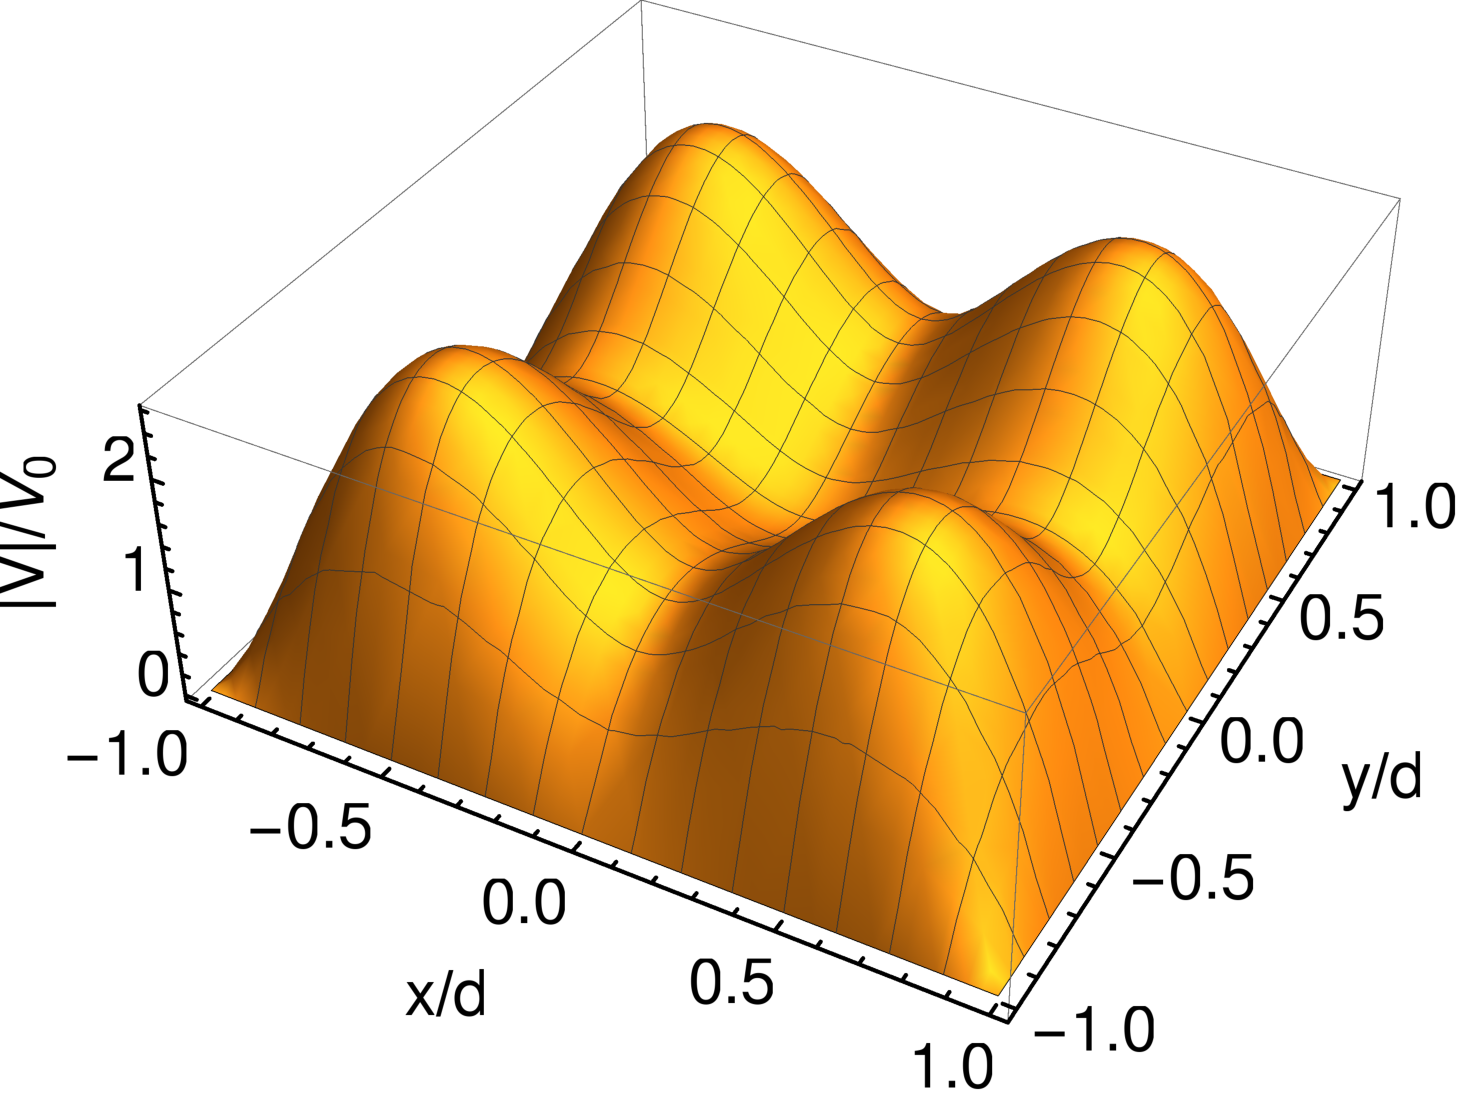
\includegraphics[width = 0.6\columnwidth]{Figures/fig_T_A_pot_abs.pdf}\\
    (b)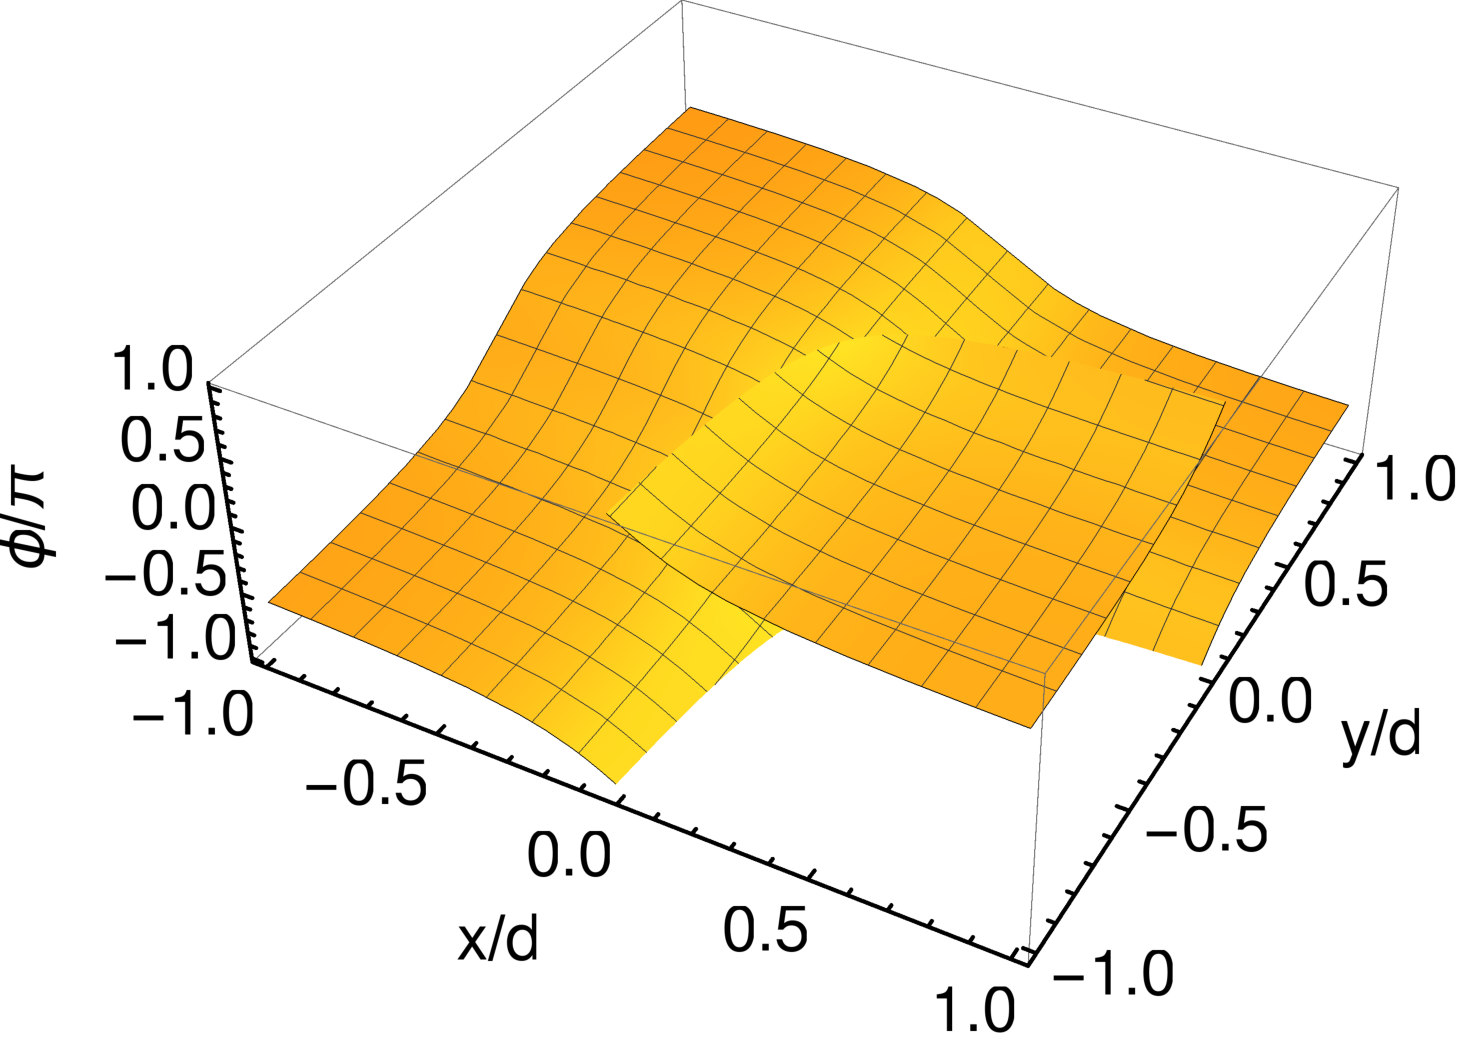
\includegraphics[width = 0.6\columnwidth]{Figures/fig_T_A_pot_arg.pdf}\\
    (c)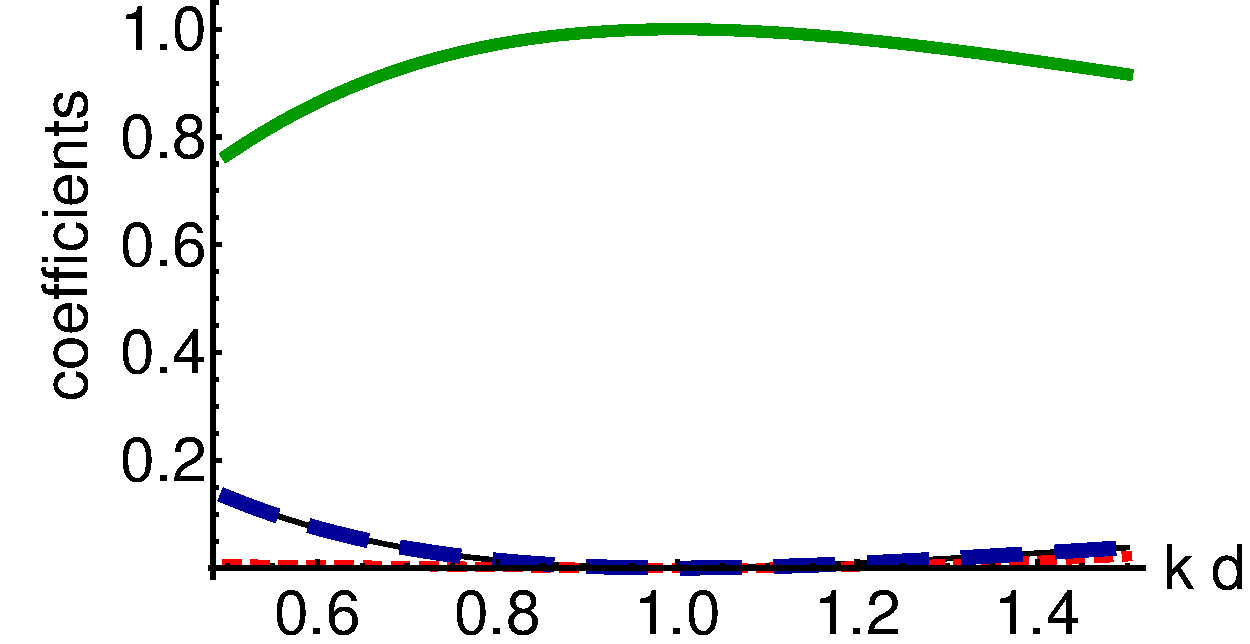
\includegraphics[width = 0.6\columnwidth]{Figures/fig_T_A_prob.pdf}
  \end{center}
  \caption{(Color online) One-way T-filter ($\cal{T/A}$, $\left|T^l\right|=1,T^r=R^l=R^r=0$) with  potential $V(x,y)=|V(x,y)|e^{i\phi(x,y)}$ set
  for $k_0 = 1/d$.
  (a) Absolute value $\left| V(x,y) \right|$;    (b) Argument $\phi(x,y)$;
  (c) Transmission and reflection coefficients:
  $\left| R^l \right|^2$ (black, solid line), $\left| T^l \right|^2$ (green, solid line),
  $\left| R^r \right|^2$ (blue, tick, dashed line), $\left| T^r \right|^2$ (red, dotted line). $V_0 = \hbar^2/(2m d^3)$.\label{fig_device_T_A}}
\end{figure}


%
%
%

\section{Designing potentials for asymmetric devices\label{sec:chapter1_examples}}

\begin{figure}
  \begin{center}
    (a) 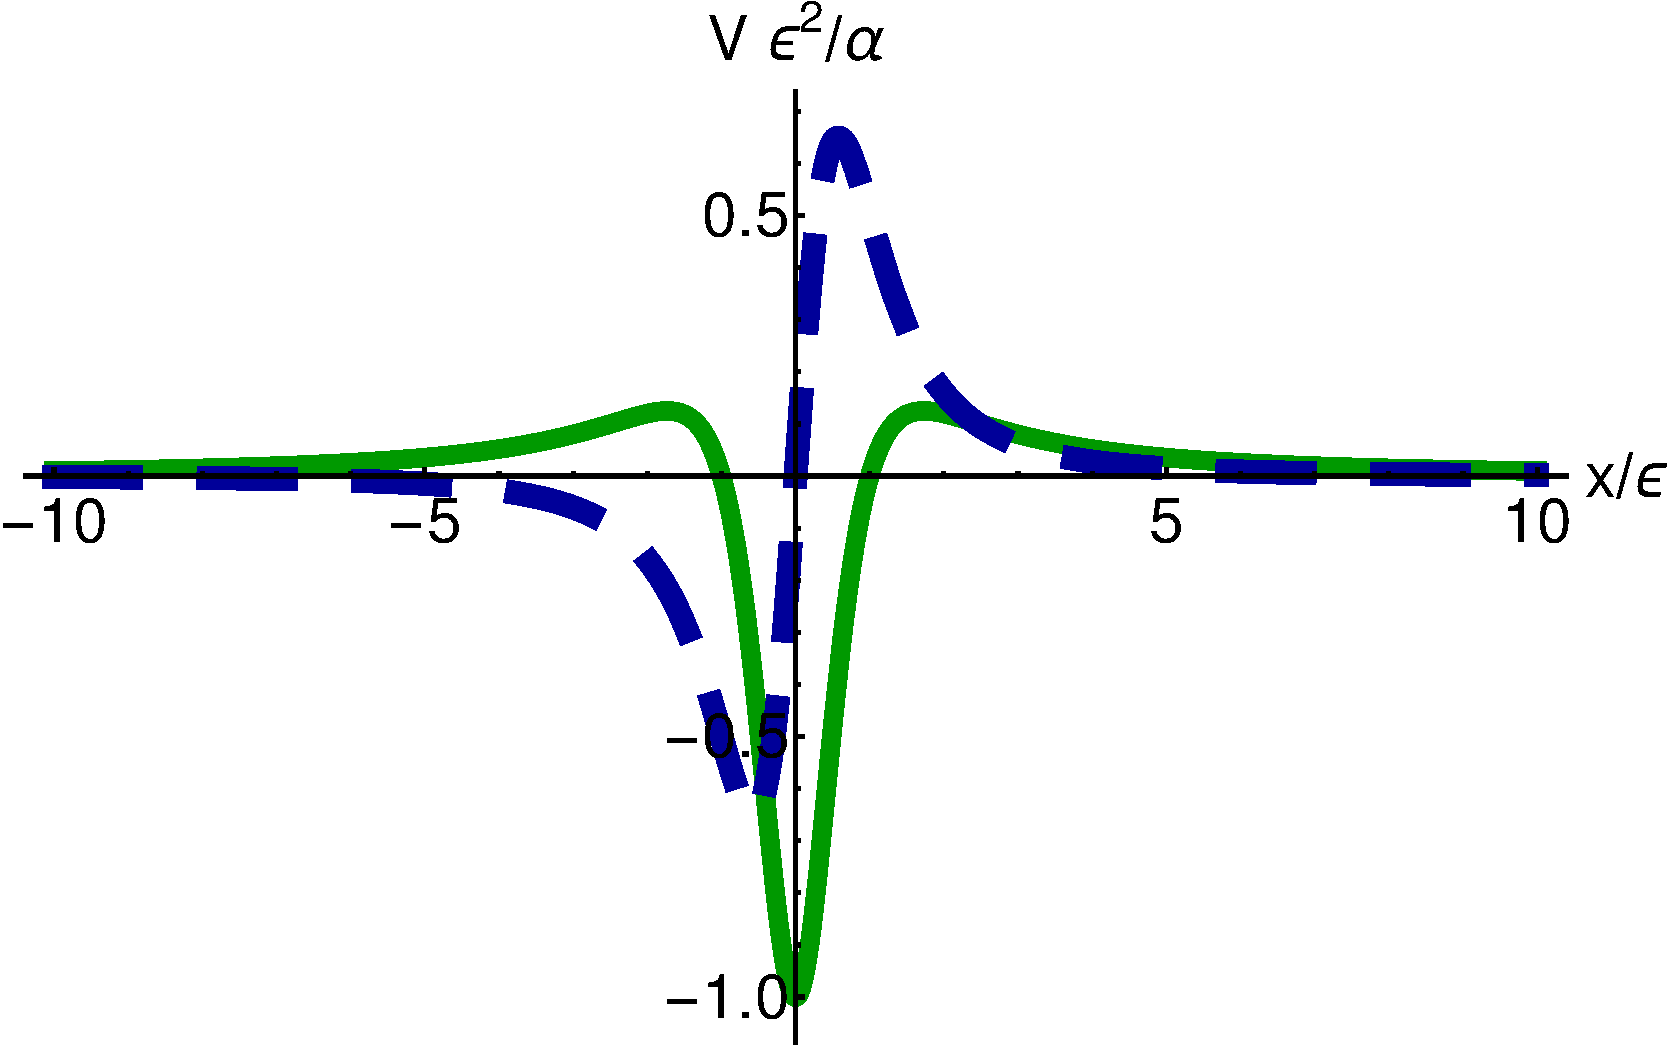
\includegraphics[width = 0.6\columnwidth]{Figures/fig_TR_T_local_pot.pdf}\\
    (b) 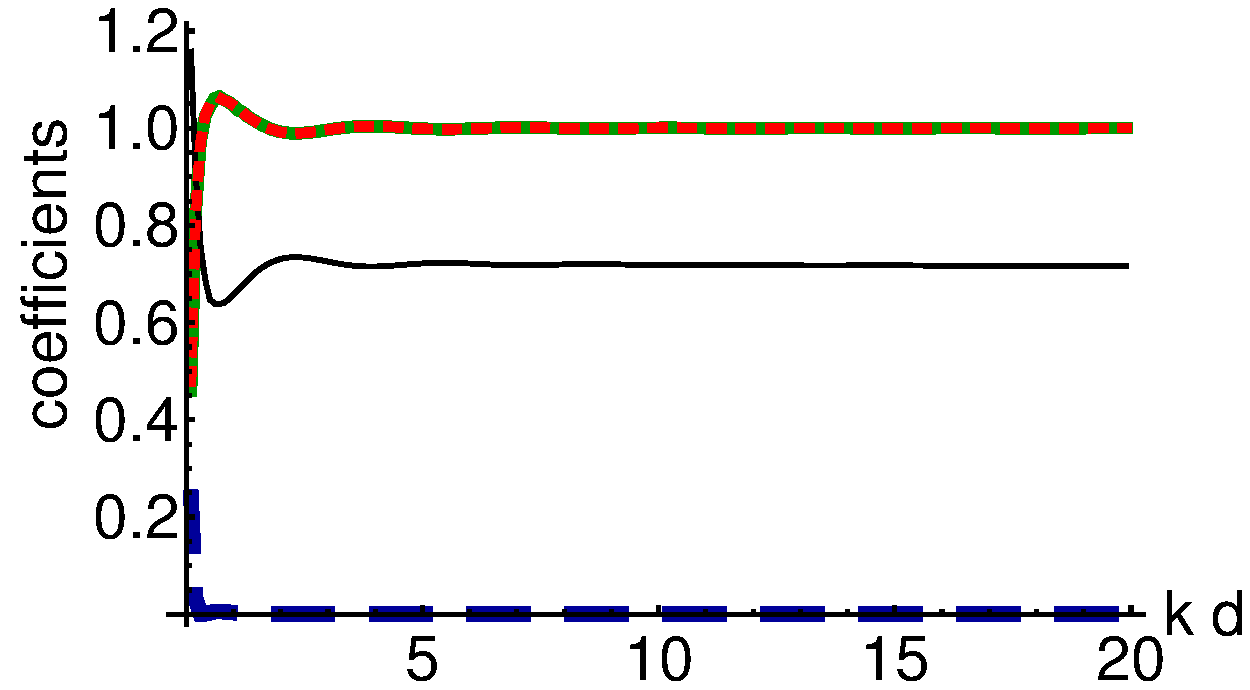
\includegraphics[width = 0.6\columnwidth]{Figures/fig_TR_T_local_prob_1.pdf}\\
    (c) 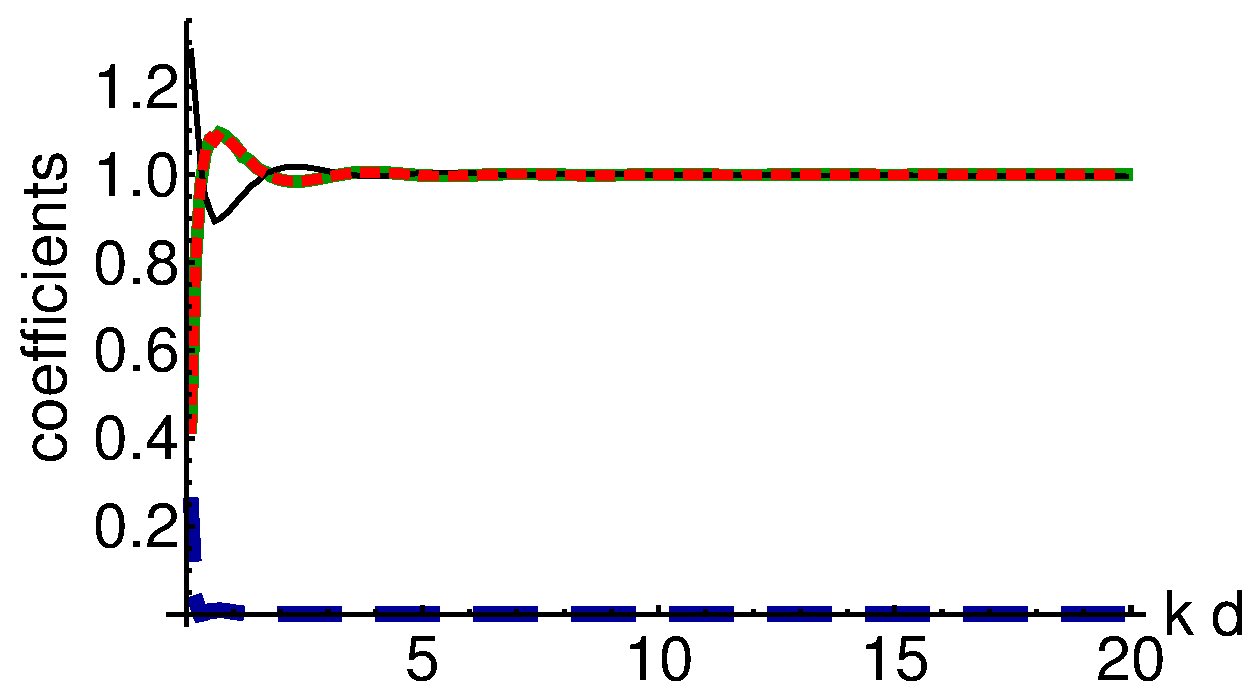
\includegraphics[width = 0.6\columnwidth]{Figures/fig_TR_T_local_prob_2.pdf}
  \end{center}
  \caption{\label{fig_reflector}(Color online) Transparent 1-way reflector with a local PT potential:
  (a) Approximation of the potential (\ref{num}), real part (green solid line), imaginary part (blue dashed line).
  (b,c) Transmission and reflection coefficients versus momentum $k d$;
  left incidence: $\left| R^l \right|^2$ (black, solid line), $\left| T^l \right|^2$ (green, solid line);
  right incidence: $\left| R^r \right|^2$ (blue, tick, dashed line), $\left| T^r \right|^2$ (red, dotted line, coincides with green, solid line).
  $\epsilon/d = 10^{-4}$.
  (b) $\alpha= 1.0 \hbar^2/(4\pi m)$ (c) $\alpha = 1.225 \hbar^2/(4\pi m)$
  (the black, solid line coincides here mostly with the red, dotted and green, solid lines).
  \label{fig_TR_T_local}}
\end{figure}


We will show  how to design non-local potentials
leading to the asymmetric devices.
For simplicity we look for  non-local potentials $V(x,y)$ with local support
that vanish  for $|x| >d$ and $|y| >d$.

To obtain the potentials for the asymmetric devices I follow an inverse scattering approach similar to \cite{Palao1998}. It starts by imposing an ansatz for the wavefunctions and the potential in the stationary Schr\"{o}dinger equation
%
\begin{eqnarray}
  \frac{\hbar^2k^2}{2m} \psi (x) = - \frac{\hbar^2}{2m} \frac{d^2}{dx^2} \psi (x)
  +\!\!\int_{-d}^d \!dy V(x, y) \psi(y).
  \label{Schroedinger}
\end{eqnarray}
%
The free parameters are fixed making use of the boundary conditions.
The form of the wavefunction incident from the left is
$\psi_l(x) = e^{i k x} + R^l e^{-i k x}$ for $x < -d$ and $\psi_l (x) = T^l e^{i k x}$ for $x > d$,
where  $k=p/\hbar$.
The wavefunction incident from the right is instead
$\psi_r(x) = e^{-ikx} T^r$ for $x < -d$ and $\psi_r (x) = e^{-i k x} + R^r e^{i k x}$ for $x > d$.

Our strategy is to assume  polynomial forms for the two wavefunctions in the interval $|x| < d$,
$\psi_l (x) = \sum_{j=0}^5 c_{l,j} x^j$ and $\psi_r (x) = \sum_{j=0}^5 c_{r,j} x^j$, and also a
polynomial ansatz of finite degree for the potential $V(x,y) = \sum_i \sum_j v_{ij} x^i y^j$.
Inserting these ansatzes in eq. (\ref{Schroedinger}) and from the conditions that $\psi_{l,r}$
and their derivatives must be continuous, all coefficients $c_{l,j}\,,c_{r,j}$ and $v_{ij}$ can be determined.
Symmetry properties of the potential can also be imposed via additional conditions on
the potential coefficients $v_{ij}$. For example we may use this method to obtain a one-way T-filter ($\cal{T/A}$) device (third device in table \ref{tab:chapter1_DevicesDescription}) with a non-local PT-pseudohermitian potential (symmetry VIII of table \ref{tab:chapter1_SymmetriesTable}) for a chosen wavevector $k = k_0$. The absolute value and argument of the resulting potential $V(x,y)$ are shown in figs. \ref{fig_device_T_A}(a) and \ref{fig_device_T_A}(b) together with its scattering coefficients as function of the incident wave vector, fig. \ref{fig_device_T_A}(c). As can be seen in fig. \ref{fig_device_T_A}(c) the imposed scattering coefficients are fulfilled exactly for the chosen wavevector. They are also satisfied approximately in a neighborhood of $k_0$. In the  Supplemental Material, Sec. II, we give further details about the construction of this potential and we work out other asymmetric devices of fig. \ref{fig:chapter1_cases}.
%
% ---------------------------------------- Asymmetric Reflection -----------------------------------
%
%
%
%

%
%%%%%%%%%%%%%%%%%%%%%%%%%%%%%%%%%%%%%%%%%%%%%%

%%%%%%%%%%%%%%%%%%%%%%%%%%%%%%%%%%%%%%%%%%%%%
%

\section{Extending the scattering asymmetry to a broad incident-momentum domain\label{sec:chapter1_extension}}
%
%
%
%
The inversion technique just described may be generalized
to extend the range of incident momenta for which the potential works by imposing additional
conditions and increasing correspondingly the number of parameters in the wavefunction ansatz,
for example we may impose that the derivatives of the  amplitudes,  in one or more orders,  vanish at $k_0$,
or  0/1 values for the coefficients not only at  $k_0$ but at a series of grid points $k_1$, $k_2$, ... $k_N$,
as in \cite{Brouard1994,Palao1998a,Palao1998,Muga2004}.

Here we put forward instead a method that provides a very broad working-window domain.
While we make formally use of the Born approximation, the exact numerical
computations demonstrate the robustness and accuracy of the approach to achieve that objective by
making use of an adjustable parameter in the potential. The very special role of the Born approximation in inverse problems has been
discussed and demonstrated in \cite{Snieder1990,Mostafazadeh2014,Horsley2015}.
Specifically we study a transparent one-way reflector ${\cal{TR/T}}$.
Our aim is now to find a local PT-symmetric potential such that asymmetric reflection results,
$T^l = T^r = 1, R^r = 0, |R^l|=1$ for a broad range of incident momenta. A similar goal
was pursued in \cite{Longhi2014} making use of a supersymmetric transformation,
without imposing $|R^l|=1$.

In the Born approximation and for a local potential $V(x)$, the reflection amplitudes take the simple form
%
\begin{eqnarray}
  R^l=-\frac{2\pi i m}{p}\langle -p|V|p\rangle,
  \;
  R^r=-\frac{2\pi i m}{p}\langle p|V|-p\rangle.
\end{eqnarray}
%
Defining the Fourier transform
%
\begin{eqnarray}
  \widetilde V (k) = \frac{1}{\sqrt{2\pi}} \int_{-\infty}^\infty dx \, V(x) e^{-i k x}
\end{eqnarray}
%
we get for $k=p/\hbar>0$:
%
\begin{eqnarray}
  R^l=-\frac{\sqrt{2\pi} i m}{k \hbar^2} \widetilde V (-2k),
  \;
  R^r=-\frac{\sqrt{2\pi} i m}{k\hbar^2} \widetilde V (2 k).
\end{eqnarray}
%
Assuming that the potential is local and PT-symmetrical, we calculate the transition coefficient
from them using generalized unitarity as
$|T|^2=1-{R^r}^*R^l$.

To build a ${\cal{TR/T}}$ device we demand:
$\widetilde V(k) = \sqrt{2\pi} \alpha k$ ($k < 0$) and $\widetilde V(k) = 0$ ($k \ge 0$).
By inverse Fourier transformation, this implies
%
\begin{eqnarray}
  V(x) &=&
  %-\alpha \frac{\partial}{\partial x} \left[P \frac{1}{x} + i \pi \delta(x) \right]
  %\nonumber\\
  %&=&
  -\alpha \frac{\partial}{\partial x} \lim_{\epsilon\to 0} \frac{1}{x - i \epsilon}
  = \alpha \lim_{\epsilon\to 0} \frac{1}{(x - i \epsilon)^2}
  \nonumber\\
  %&=& \alpha \lim_{\epsilon\to 0} \frac{(x + i \epsilon)^2}{(x^2 + \epsilon^2)^2}\\
  &=& \alpha \lim_{\epsilon\to 0} \left[\frac{x^2 - \epsilon^2}{(x^2 + \epsilon^2)^2} + i
  \frac{2 x\epsilon}{(x^2 + \epsilon^2)^2}\right],
  \label{num}
\end{eqnarray}
%
which is indeed a local, $PT$-symmetric potential for $\alpha$ real.
$\alpha$ is directly related to the reflection coefficient, within the Born approximation,
$R^l = 4 \pi i m \alpha/\hbar^2$. As the Born approximation may differ from exact results
we shall keep $\alpha$ as an adjustable parameter
in the following.

In a possible physical implementation, the potential in eq. (\ref{num}) will
be approximated by keeping a small finite $\epsilon>0$, see fig. \ref{fig_TR_T_local}(a).
%\begin{eqnarray}
%V(x) = \alpha \left[\frac{x^2 - \epsilon^2}{(x^2 + \epsilon^2)^2} + i
%\frac{2 x\epsilon}{(x^2 + \epsilon^2)^2}\right],
%\end{eqnarray}
%with a finite, small $\epsilon>0$.
Then, its Fourier transform is
$\widetilde V(k) = \sqrt{2\pi} \alpha k e^{\epsilon k}$ ($k < 0$) and $\widetilde V(k)=0$ ($k \ge 0$).
In figs. \ref{fig_TR_T_local}(b) and (c), the resulting coefficients for $\epsilon/d=10^{-4}$ and  two different values
of $\alpha$ are shown.  These figures have been calculated by
numerically solving the Schr\"odinger equation exactly.
% and demonstrate that
%$\alpha$ can indeed  be adjusted so that $\left| R^l \right|^2 \approx 1$.
Remarkably, the Born approximation contains all the information required to build the required potential shape
up to a global factor.  Such a prominent role of the Born approximation in inverse problems has been noted
in different applications \cite{Snieder1990,Mostafazadeh2014,Horsley2015}. For a range of $\alpha$, the potential gives $|R^r|\approx 0$, a nearly constant $|R^l|^2$, and
$|T^r|= |T^l|\approx1$  in a broad $k$-domain, see fig. \ref{fig_TR_T_local}(b). Adjusting  the value of $\alpha$, fig. \ref{fig_TR_T_local}(c),
sets $|R^l|\approx 1$ as desired.
%
%Remarkably, except for very low $k$,
%the potential is reflectionless from the right
%and provides full transmission independently of $\alpha$. As well, $|R^2|^2$ stays constant with respect to $k$ for different $\alpha$,
%so that that up to the adjustable parameter the Born approximation provides in fact the required potential shape, a surprising
%in inverse problems \cite{Snieder1990,Mostafazadeh2014,Horsley2015}.
%Figure \ref{fig_TR_T_local}(c) demonstrates that $\alpha$ can indeed be adjusted so that the  potential works
%as intended, i.e., as a transparent one-way reflector,  for a very broad range of $k$ values.

%
%
%
%
%
\section{Discussion\label{sec:chapter1_Discussion}}
%
%
Scattering asymmetries are necessary to develop technologically relevant devices such
as one-way mirrors, filters and  barriers, invisibility cloaks, diodes, or Maxwell demons.
So far much effort has been devoted to build and apply local PT-symmetric potentials but the possible scattering asymmetries with them are
quite limited. We find that six  device types with asymmetric scattering are possible
when imposing $0$ or $1$ scattering coefficients.
PT-symmetry can only realize one of them, but this symmetry  is just one among eight possible symmetries of complex non-local potentials.
The eight symmetries arise from the discovery that Klein's four-group
$\{1, \Pi, \Theta, \Theta\Pi\}$, combined with two possible relations among the Hamiltonian, its adjoint,
and the symmetry operators of the group, eqs. (1) and (2),
produce all possible  equalities among potential matrix elements after the action of complex conjugation, coordinate inversion, the identity, and transposition.
In other words, to have all possible such equalities, the conventional definition of a symmetry $A$ in terms of its commutation with the Hamiltonian $H$ is not enough, and $A$-pseudohermiticity must be considered as well on the same footing.
Extending the concept of what a symmetry is for complex, non-local potentials is
a fundamental, far-reaching step of this work.
This group theoretical analysis and classification is not only esthetically pleasing, but also of practical importance, as it reveals
the underlying structure and span of the possibilities available in principle to manipulate the asymmetrical response of a potential
for a structureless particle.

We provide a potential for a One-way T-filter ($\mathcal{T}/\mathcal{A}$) and a PT potential for a transparent One-way reflector ($\mathcal{T}\mathcal{R}/\mathcal{T}$) that works in a broad domain of incident momenta. Although the present theory is for the scattering of quantum particles, the analogies between quantum physics and optics suggest to extend the concepts and results for optical asymmetric devices.
%
